\documentclass{beamer}

\usepackage[utf8]{inputenc}
\usepackage{tikz}
\usepackage{caption}
\usepackage{subcaption}
\usepackage[natbib, style=authoryear,backend=biber]{biblatex}
\usepackage{amsmath}
\usepackage[linesnumbered,lined,commentsnumbered,noend,noline]{algorithm2e}
\usepackage{pgfplots}
%\usepackage{enumitem}

\usetikzlibrary{arrows, arrows.meta}

\newcommand{\RR}{\mathbb{R}}
\newcommand{\CC}{\mathbb{C}}
\newcommand{\ZZ}{\mathbb{Z}}
\newcommand{\QQ}{\mathbb{Q}}
\newcommand{\NN}{\mathbb{N}}
\newcommand{\EE}{\mathbb{E}}
\newcommand{\PP}{\mathbb{P}}
\newcommand{\BB}{\mathbb{B}}

\DeclareMathOperator{\PartialSpanner}{\textsc{PartialSpanner}}
\DeclareMathOperator{\Cover}{\textsc{Cover}}
\DeclareMathOperator{\Sample}{\textsc{Sample}}
\DeclareMathOperator{\ball}{ball}
\DeclareMathOperator{\InTree}{InTree}
\DeclareMathOperator{\OutTree}{OutTree}
\DeclareMathOperator{\InOutTrees}{InOutTrees}

\setbeamercolor{block body alerted}{bg=alerted text.fg!10}
\setbeamercolor{block title alerted}{bg=alerted text.fg!20}
\setbeamercolor{block body}{bg=structure!10}
\setbeamercolor{block title}{bg=structure!20}
\setbeamercolor{block body example}{bg=green!10}
\setbeamercolor{block title example}{bg=green!20}
\setbeamertemplate{blocks}[rounded][shadow]

\newtheorem{proposition}{Proposition}

\title{Randomization in Recent Progress on \\ Traveling Salesman Problem}
\author{Yuchong Pan}
\institute{MIT 6.842}
\date{\today}

\begin{document}
  \frame{\titlepage}

  \begin{frame}
  
    \centering
    \includegraphics[width=\textwidth]{figures/mtwashington.png}
  
  \end{frame}

  \begin{frame}

    \centering
    
\includegraphics[width=\textwidth]{figures/tuckermans.png}
  
  \end{frame}

  \begin{frame}
    \frametitle{Metric Traveling Salesman Problem}
  
    \begin{block}{Metric Traveling Salesman Problem (TSP)}
      \begin{tabular}{rl}
        {\bf Input:} & a set $V$ of vertices and pairwise symmetric costs \\
        & $c : V \times V \to \RR_+$ which satisfies the triangle inequality \\
        {\bf Output:} & a shortest tour that visits each vertex exactly once
      \end{tabular}
    \end{block}

    \pause

    \bigskip

    \begin{quote}
      It belongs to the most seductive problems in combinatorial optimization, thanks to a blend of complexity, applicability, and appeal to imagination.

      \begin{flushright}
        --- Lex Schrijver
      \end{flushright}
    \end{quote}
  
  \end{frame}

  \begin{frame}
    \frametitle{The Christofides-Serdyukov Algorithm}
  
    \begin{block}{The Christofides-Serdyukov Algorithm (1976, 1978)}
      \begin{algorithm}[H]
        $T \leftarrow \text{a minimum spanning tree of $G$}$ \\
        $O \leftarrow \{ v \in V : \deg_T(v) \text{ is odd} \}$ \\
        $M \leftarrow \text{a minimum-weight perfect matching in $G[O]$}$ \\
        find a Eulerian tour in $T \cup M$ \\
        shortcut repeated vertices to form a Hamiltonian tour
      \end{algorithm}
    \end{block}

    \pause

    \bigskip

    {\bf approximation ratio: } $3/2$

    \pause

    \medskip

    {\bf the ``$4/3$-conjecture''}
  
  \end{frame}

  \begin{frame}
    \frametitle{... 45 Years Later}
  
    \pause

    \begin{theorem}[Karlin, Klein and Oveis Gharan, 2021]
      For some absolute constant $\varepsilon > 10^{-36}$, there exists a {\bf randomized} algorithm that outputs a tour with expected cost at most $3/2 - \varepsilon$ times the cost of the optimum solution.
    \end{theorem}

    \pause

    \bigskip

    \begin{itemize}
      \item[$\circ$] We assume that the metric is a {\bf graph metric}, i.e., there exists an unweighted graph where the metric is the shortest path metric of that graph. This special case is due to Oveis Gharan, Saberi and Singh (2011). \pause
      \item[$\circ$] To focus on the randomization part of the proof, we assume that all proper cuts with respect to $x$ have size at least $2 + \varepsilon$. In the general case, we exploit the structure of near-min-cuts, called the {\bf deformable polygon representation} developed by Bencz\'ur and Goemans.
    \end{itemize}
  
  \end{frame}

  \begin{frame}
    \frametitle{Subtour Elimination LP}
  
    \begin{alignat*}{4}
      & \text{minimize} \qquad & \sum_{u, v \in V} x_{\{ u, v \}} c(u, v) \\
      & \text{subject to} \qquad & \sum_{\{ u, v \} \in \delta(S)} x_{\{ u, v \}} &\geq 2 && \qquad \forall S \subsetneq V, S \neq \emptyset \\
      & & \sum_{\{ u, v \} \in \delta(\{ v \})} x_{\{ u, v \}} &= 2 && \qquad \forall v \in V \\
      & & x_{\{ u, v \}} &\in [0, 1] && \qquad \forall u, v \in V
    \end{alignat*}
  
  \end{frame}

  \begin{frame}
    \frametitle{$O$-Joins}
  
    \begin{definition}[$O$-joins]
      A set $F \subset E$ is an {\bf $O$-join} if every vertex $v \in O$ has odd degree in $F$, and every other vertex has even degree in $F$.
    \end{definition}

    \pause

    \medskip

    \begin{figure}[H]
      \centering
      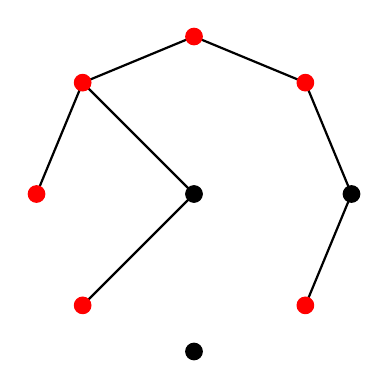
\begin{tikzpicture}
        \draw[thick] (225:2) -- (0:0) -- (135:2) -- (180:2);
        \draw[thick] (135:2) -- (90:2) -- (45:2) -- (0:2) -- (315:2);
        \draw[black, fill=black] (0:2) circle (3pt);
        \draw[red, fill=red] (45:2) circle (3pt);
        \draw[red, fill=red] (90:2) circle (3pt);
        \draw[red, fill=red] (135:2) circle (3pt);
        \draw[red, fill=red] (180:2) circle (3pt);
        \draw[red, fill=red] (225:2) circle (3pt);
        \draw[black, fill=black] (270:2) circle (3pt);
        \draw[red, fill=red] (315:2) circle (3pt);
        \draw[black, fill=black] (0:0) circle (3pt);
      \end{tikzpicture}
    \end{figure}

    \pause

    \medskip

    {\bf observation:} an $O$-join is a union of paths connecting red vertices
  
  \end{frame}

  \begin{frame}
    \frametitle{$O$-Joins}
  
    \begin{theorem}[Edmonds and Johnson, 1973]
      For any graph $G = (V, E)$ with edge costs $c : E \to \RR_+$ and for any $O \subset V$ with $|O|$ even, the minimum cost of an $O$-join equals the optimum value of the following LP:
      \begin{alignat*}{4}
        & \text{minimize} \qquad & c(y) \\
        & \text{subject to} \qquad & y(\delta(S)) &\geq 1 && \qquad \forall S \subsetneq V, |S \cap O| \text{ odd} \\
        & & y_e &\geq 0 && \qquad \forall e \in E
      \end{alignat*}
    \end{theorem}
  
  \end{frame}

  \begin{frame}
    \frametitle{A Randomized Rounding Algorithm}

    \begin{definition}[$\lambda$-uniform distributions]
      For $\lambda: \EE \to \RR_{\geq 0}$, a {\bf $\lambda$-uniform} distribution $\mu_\lambda$ on spanning trees on a graph $G$ satisfies that for any spanning tree $T$,
      $$ \PP_\mu[T] \propto \prod_{e \in E(T)} \lambda_e. $$
    \end{definition}
  
    \begin{block}{Algorithm (Oveis Gharan, Saberi and Singh, 2011)}
      \begin{algorithm}[H]
        $x \leftarrow \text{an optimal solution to the subtour elimination LP}$ \\
        $\mu \leftarrow \text{a $z$-uniform distribution with marginal $z = (1 - 1/n) x$}$ \\
        $T \sim \mu$ \\
        $O \leftarrow \text{set of odd degree vertices in $T$}$ \\
        find a minimum cost $O$-join $F$ \\
        \Return{$T \cup F$}
      \end{algorithm}
    \end{block}
  
  \end{frame}

  \begin{frame}
    \frametitle{A (Very) High Level Idea}

    \pause
  
    \begin{enumerate}
      \item[$\circ$] $\EE[c(T)] = \sum_{e \in E} c(e) z(e) = c(z) = (1 - 1/n) c(x)$. \pause
      \item[$\circ$] First, let's see $c(F) \leq c(x)/2$. \pause
      \item[$\circ$] Let $y(e) = x(e)/2$ for all $e \in E$. \pause
      \item[$\circ$] Since $x(\delta(S)) \geq 2$ for all proper $S \subset V$, then $y(\delta(S)) \geq 1$. \pause
      \item[$\circ$] Hence, $c(F) \leq c(y) = c(x)/2$. \pause
      \item[$\circ$] However, we only need to satisfy $y(\delta(S)) \geq 1$ for all $S \subset V$ with $|S \cap O|$ odd. \pause
      \item[$\circ$] The idea is to use the randomness of $T$ to assign a slightly value $y(e) = (1/2 - \varepsilon') x(e)$ to some of the edges (with constant probability) while preserving the feasibility of $y$.
    \end{enumerate}
  
  \end{frame}

  \begin{frame}
    \frametitle{Even Edges, Good Edges}
  
    \begin{definition}[even edges]
      An edge is {\bf even} if both of its endpoints have degree $2$ in $T$.
    \end{definition}

    \pause

    \begin{definition}[good edges]
      An edge $e$ is {\bf good} if
      $$ \PP[\text{$e$ is even}] \geq \gamma, $$
      for some constant $\gamma$ to be determined later.
    \end{definition}
  
  \end{frame}

  \begin{frame}
    \frametitle{Even Edges, Good Edges}
  
    \begin{lemma}
      Suppose that every edge $e$ is good. Then
      \vspace{-10pt}
      $$ \EE[c(F)] \leq \left(\frac{1}{2} - \Omega(\varepsilon \cdot \gamma)\right) c(x). $$
    \end{lemma}

    \pause

    \begin{proof}
      \begin{itemize}
        \item[$\circ$] For any $e \in E$, let
        \vspace{-10pt}
        $$ y(e) = \left\{
          \begin{array}{ll}
            x(e)/(2 + \varepsilon), & \text{if $e$ is even}, \\
            x(e)/2, & \text{otherwise}.
          \end{array}
        \right. $$
        \vspace{-15pt}
        \pause
        \item[$\circ$] For any proper $S$, we have $y(\delta(S)) \geq x(\delta(S))/(2 + \varepsilon) \geq 1$. \pause
        \item[$\circ$] If $v$ has odd degree, then $y(\delta(\{ v \})) = x(\delta(\{ v \})) = 1$. \pause
        \item[$\circ$] Since every edge is good,
        \vspace{-10pt}
        $$ \EE[c(y)] \leq \sum_{e \in E} \frac{x(e)}{2} \left(1 - \PP[\text{$e$ even}] \frac{\varepsilon}{4}\right) \leq \left(\frac{1}{2} - \Omega(\varepsilon \cdot \gamma)\right) c(x). $$
        \vspace{-20pt}
      \end{itemize}
    \end{proof}
  
  \end{frame}

  \begin{frame}
    \frametitle{Existence of Good Edges (Very, Very High Level)}

    \pause
  
    \begin{itemize}
      \item[$\circ$] Trivally, we cannot expect a tree to have an even number of edges in every cut. \pause
      \item[$\circ$] However, using randomness, we can expect to have an even number of edges in at least $1/3$ of the cuts. \pause
      \item[$\circ$] The crux of the proof is that the degree distribution of a vertex equals the sum of independent Bernoulli random variables $B_1, \ldots, B_m$ (using real stable polynomials). \pause
      \item[$\circ$] It remains to answer what is the minimum possible value of $\PP[B_1 + \ldots + B_m = 2]$.
    \end{itemize}

    \pause

    \begin{theorem}[Hoeffding, 1956]
      For any Bernoulli's $B_1, \ldots, B_n$ with success probabilities $p_1, \ldots, p_n$ and any $g : \RR \to \RR$, $\EE[g(B_1 + \ldots + B_m)]$ is minimized when $p_1, \ldots, p_m \in \{ 0, p, 1 \}$ for some fixed $p$.
    \end{theorem}
  
  \end{frame}

\end{document}